\subsection{Марковские цепи}
Вспоминаем задачку с Петей, монеткой и кинотеатром и визуализируем в виде ориентированного графа.
\begin{center}
    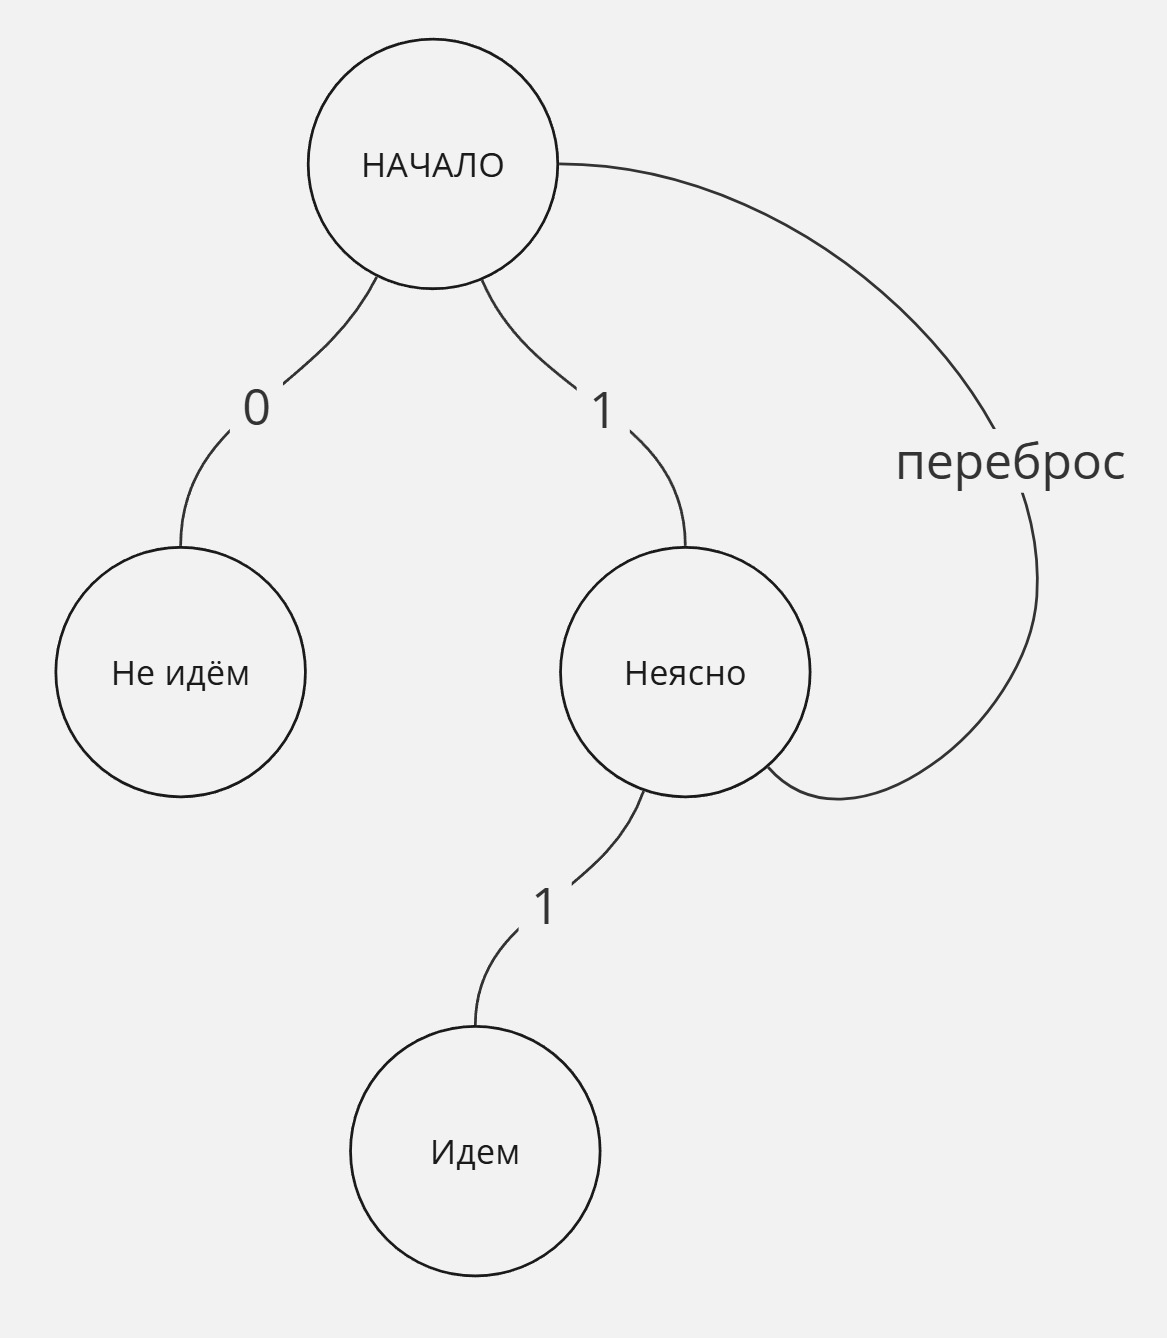
\includegraphics[width = 7cm]{assets/5_1_1.jpg}
\end{center}
Заметим, что результаты нам не особо важны, важны только вероятности, перерисуем и дополнительно заведём ограничение на сумму значений вероятностей исходящих из вершины: сумма должна всегда должна быть равна единичке.
\begin{center}
    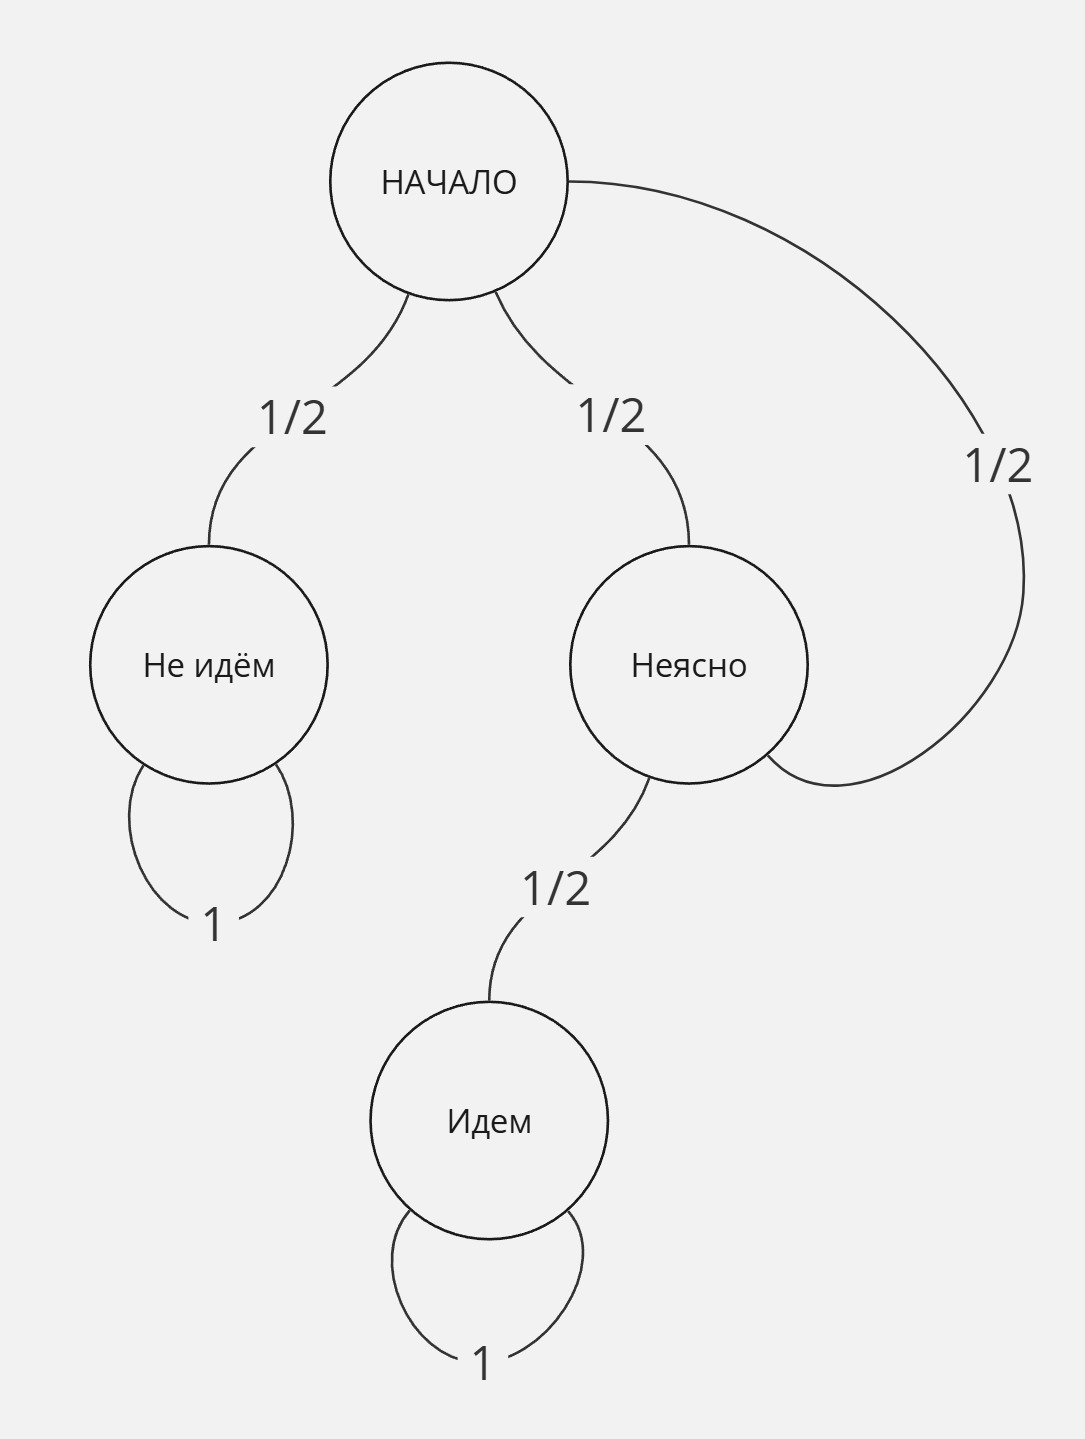
\includegraphics[width = 7cm]{assets/5_1_2.jpg}
\end{center}
Давайте для такого графа введём определение.
\newpage
\deff{Марковской цепью} называется ориентированный граф с конечным числом вершин, у которых на исходяших рёбрах написаны вероятности, причём для каждой вершины верно, что сумма этих рёбер равна единице. Введём ещё парочку определений.



Вершина называется \deff{полглощающей} если из неё исходит только петля.




Обозначим векторами $b^{(t)}_i = P(\xi_t = i)$, $b^{t} = (b_1^{(t)}, \ldots, b_n^{(t)})$ - распределение $\xi_t$. 
\newline
Давайте с такими данными построим матричку $P_{n\times n}$, где значение в ячейке -- это вероятность перейти из $i$-той вершины в $j$-тую. Разберём пример:
\newline 
\[
P = 
\begin{pmatrix}
0 & \dfrac{1}{2} & \dfrac{1}{2} & 0 \\
0 & 1 & 0 & 0 \\
\dfrac{1}{2} & 0 & 0 & \dfrac{1}{2} \\
0 & 0 & 0 & 1
\end{pmatrix}
\]
Хочется что-то с этой матрицей начать делать, начнём же:


\thmm{Лемма 1.} $b^{(t + 1)} = b^{(t)}P$

     \textbf{Доказательство:}
      $$ b_i^{(t + 1)} = P(\xi_{t+1} = i) = \sum_{j = 1}^n P(\xi_{t+1} = i \quad\&\quad \xi_t = j)P(\xi_t = j) = \sum_{j = 1}^{n}b_{j}^{(t)}P_{ji} = (b^{(t)}P)_i$$
\hfill Q.E.D.

По коэффициенту очевидности $b^{(t)} = b^{(0)}P^t$,  проверяйте сами

МЦ называется \deff{поглощающей}, если $\forall u \ \exists$ путь такой, что $u \rightarrow$ поглощаемая вершина

Введём отношение эквивалентности такое, что $u \sim v $ если $\exists$ пусть $u \rightarrow v$ и наоборот.

Можем заметить, что у нас образуется разбиение на классы эквивалентности, рассмотрим $[1 ;n]\ /\sim$ ,  
$\tilde{u}$ -- класс эквивалентности 




$\tilde{u}$ -- \deff{эргодический класc}.
тем самым мы можем разделять задачи на две части: на наблюдение свойств в самом классе и между классами.


МЦ -- \deff{эргодическая}, если в ней ровно 1 эргодический класс

Эргодический класс называется \deff{периодическим}, если $\exists d > 1$, что размер любого цикла делится на $d$ -- сама $d$ называется \deff{периодом}, очевидно, что период -- нод длин всех циклов

\thmm{Теорема о классификации Марковских Цепей.}

     В любой МЦ есть поглощающий эргодический класс, вероятность того, что МЦ окажется в одном таких классов стремится к единице

     Вторая часть, я не могу разобрать свой почерк, на паре мы это не доказывали пока
    
     \textbf{Доказательство:}
\[
P = 
\left(
\begin{array}{c|c}
    Q & R \\ \hline
    \mathbf{0} & E
\end{array}
\right)
\text{, где } Q_{m \times m} \,, R_{m \times (n -m)}, \text{ где } m \text{ -- это непоглощающие эргодические классы }
\]
тогда каждый вектор $b^{(t)}$ делится на две части: первые m координат обзовём $a^{(t)}$, вторые назовём  $c^{(t)}$. $a_i^{(t)} = P(\xi_t = i)$, где $i$ непоглощающая

\thmm{Лемма 2.}
$a^{(t)} = a^{(0)}Q^t$, лемма очевидна просто взгляните, на то, как умножается вектор на матрицу

\thmm{Лемма 3.}
$Q^k \xrightarrow[k\rightarrow+\infty]{}\mathbf{0}$
\begin{quote}
    
     \textbf{Доказательство:}
     
     Для того, чтобы найти предел матрицы нам нужно ввести норму, норму введём такую
     $|A| = max_{ij}|a_{ij}|$, сами докажете, что это норма, не маленькие.

     Тогда матрица стремится к нулю, если её норма стремится к нулю, наша задача показать, что 
     $Q^n \xrightarrow[n\rightarrow +\infty]{} \mathbf{0}$

     Пусть L - максимальная длина кратчайшего пути от i до поглощения, давайте посмотрим чему равно 
     $X = Q^L$, рассмотрим $x_{ij} = \sum_{k_1, k_2, .. k_{l - 1}}q_{ik_1}q_{k_1, k_2}q_{k_2, k_3} q_{l-1, j}$. Чему равна эта сумма, неясно, каждое из этиъ произведений -- это вероятность пройти оп пути длиной ровно $L$ от вершины $i$ до $j$, давайте рассмотрим такую сумму $$\sum_{j\text{-не погл}}x_{ij} = \sum_{k_1, k_2, .. k_{l - 1}, j}q_{ik_1}q_{k_1, k_2}q_{k_2, k_3} q_{l-1, j} = \delta < 1$$
     Меньше единицы оно потому, что мы смотрим не на все пути, а лишь на часть. Посмотрим на матричку:
     \begin{multline*}
     \displaystyle Q_{ij}^n =(Q^L Q^{n-L})_{ij} = \sum_k Q^L_{ik}Q_{kj}^{n-L} \leq (\sum_k Q_{i, k}^L)|Q^{n - L}| \leq \delta|Q^{n - L}| \text{ т.к. } |Q^{n}| <= \delta^{\lfloor n/l \rfloor}
     \\ \text{ то наше выражение стремится к нулю}
     \end{multline*}

     Лемму доказали, стало быть, и теоремка доказана.
\end{quote}




Передём к вычислительным моментам, мы хотим понять, где мы поглотимся.
Найдём мат. ожидание времени до поглощения
Давайте введём $T$ -- случайная величина : число шагов до поглощения, тогда 
$T = \sum_{i=1}^mT_i$ $T_i$ -- число посещений $i$-го состояния

$T_i = \sum_{j = 0}^{\infty}T_{ij}$ 

\[
T_{ij} = 
\begin{cases}
1, & \text{если на шаге } j \text{ марковская цепь находится в состоянии } i, \\
0, & \text{иначе.}
\end{cases}
\]

$$P(\text{м.ц на шаге $j$ в состоянии $i$} = (a^0 Q^j)_i$$


$$ET = \sum_{i=1}^nET_i = \sum_{i = 1}^m\sum_{j = 0}^{\infty}ET_{ij} = \sum_{i = 1}^m\sum_{j = 0}(a^0 Q^j)_i$$

Воспользуемся линейной алгеброй, т.к. сумма матриц перестановочна относительно взятия $i$-го компонента
$$\sum_{i = 1}^m\sum_{j = 0}^{\infty}(a^0 Q^j)_i = \sum_{i = 1}^m(\sum_{j = 0}^{\infty}a^0 Q^j)_i$$
т.к. $a^0$ не зависит от $j$ 
$$\sum_{i = 1}^m(\sum_{j = 0}^{\infty}a^0 Q^j)_i = \sum_{i = 1}^m a^0 (\sum_{j = 0}^{\infty} Q^j)_i$$

\hfill Q.E.D.

\thmm{Лемма}
$\sum_{j = 0}^{\infty}Q^j = (I - Q)^{-1}$

\textbf{Доказательство:}
    $$(E-Q)(E+Q+Q^2+Q^3+\ldots) = E - Q + Q - Q^2 + Q^2 + \ldots - Q^{n+1}$$ $$= E - Q^{n+1} = E \text{ т.к. $Q $ стремится к нулю} $$
\hfill Q.E.D.

\deff{Фундаментальная матрица полглощения м.ц.} -- это $N = (I - Q)^{-1}$

\begin{multline*}
P(\text{погл в $j$}) = \sum_i^m P(\text{погл в $j$ из $i$}) P(\text{$j$ перед поглощением}) = \sum_t^{\infty}\sum_{i=1}^m P(\text{погл в $j$ из $i$ в $t$}) \\= P(\text{быть в i в момент вермени t}) = a^0NR
\end{multline*}


Откуда получаем 2 крутые и очень полезные в дальнейшем формулы: